\documentclass[slidestop,compress,mathserif]{beamer}
\usepackage{graphics,graphicx}
\usepackage{latexsym}
%usepackage[dvipsnames,usenames]{color}
%\usepackage{movie15}
%\usepackage{hyperref}
%\usepackage{multimedia}
\usepackage[latin1]{inputenc}
\usepackage[english]{babel}
\usepackage{amsmath}
\usepackage{amssymb}
\usepackage{amsthm}
%\usepackage{bbm}
%\usepackage[all]{xy}
\usepackage{algpseudocode}
%\usepackage[dvipdfmx]{media9}
%\usepackage{geometry}
%\geometry{verbose,letterpaper}

\newcommand{\bi}{\begin{itemize}}
\newcommand{\ei}{\end{itemize}}
\newcommand{\bis}{\begin{itemize}[<+->]}
\newcommand{\eis}{\end{itemize}}

\newcommand{\indep}{\ensuremath{\perp\mkern -10mu \perp}}
\newcommand{\notindep}{\ensuremath{\perp\mkern -10mu \perp \mkern -17mu \not \mkern 17mu}} % statistically dependent


\usetheme{default}
\mode<presentation>
{
  \usetheme{Boadilla}
  \usecolortheme{beaver}
  % \usetheme{Warsaw}
  % or ...

  \setbeamercovered{transparent}
  % or whatever (possibly just delete it)
}


%\usepackage[algoruled,linesnumbered]{algorithm2e}
\usepackage{algorithm}
%\usepackage{algorithmic}

\title[Probabilistic Graphical models]
{Probabilistic Graphical models}

\subtitle
{Machine Learning (MIIS 2021-2022)} % (optional)

\author[\hspace{10cm}]{
  Vicen\c{c}~G\'omez}
  %Hilbert J~Kappen\inst{1}}%\inst{1,2}}

\institute[Machine Learning (MIIS)] % (optional, but mostly needed)
{ 
Department of Information and Communication Technologies \\
Universitat Pompeu Fabra \\
}
\date[] % (optional)
 
\subject{Talks}
% This is only inserted into the PDF information catalog. Can be left
% out. 

% If you have a file called "university-logo-filename.xxx", where xxx
% is a graphic format that can be processed by latex or pdflatex,
% resp., then you can add a logo as follows:
%\pgfdeclareimage[height=0.5cm]{university-logo}{images/upf.jpg}
%\logo{\pgfuseimage{university-logo}}

% Delete this, if you do not want the table of contents to pop up at
% the beginning of each subsection:
\AtBeginSubsection[]
{
  \begin{frame}<beamer>
    \frametitle{Outline}
    \tableofcontents[currentsection,currentsubsection]
  \end{frame}
}

% \pgfdeclareimage[height=0.8cm]{university-logo}{barcelona_media_logo}
% \logo{\pgfuseimage{university-logo}}



% \title{Graphical model inference and multi-agent optimal control}
% \author{Vicen\{c}}
% \institute{Radboud University, Nijmegen}
% \date{May 24, 2013}
% 
% \logo{\includegraphics[height=1cm]{/Users/bertkappen/doc/styles/COMPLACS_LOGO_RGB.pdf}}

\begin{document}

\begin{frame}
  \titlepage
\end{frame}

\begin{frame}
  \frametitle{Outline}
  \tableofcontents%[pausesections]
  % You might wish to add the option [pausesections]
\end{frame}

\section{Introduction to probabilistic Graphical Models}

\begin{frame}
	\frametitle{Introduction to probabilistic graphical models}
	\framesubtitle{Motivation}
%$$P(x,y)=P(x|y)P(y)=P(y|x)P(x)$$
    Most of the material of these slides has been taken
    from :
    \begin{itemize}
    \item Chapter 8 of C. Bishop's book
    \item D. Mackay's book
    \item Tutorial on Graphical Models of Z. Ghahramani (MLSS 2012)
    \end{itemize}
    \end{frame}



\begin{frame}
	\frametitle{Introduction to probabilistic graphical models}
	\framesubtitle{Motivation}

    \bi
    \item Unifying language to express many existing problems
    \item Intersection of many different scientific areas 
    \begin{itemize}
    \item probability theory
    \item computer science
    \item decision theory
    \item optimization
    \item ...
    \end{itemize}
    \item Examples of applications:
medical and fault diagnosis, image understanding, reconstruction of
biological networks, speech recognition, natural language processing, decoding
of messages sent over a noisy communication channel, robot navigation, and many
more
    \ei
%    \footnote{
%\fontsize{9pt}{7.2}\selectfont
%    \begin{description}
 %   \item
% Material : Chapter 8 C. Bishop's book, D. Mackay's book, M. Jordan notes
    %\end{description}
%    }
\end{frame}

\begin{frame}
	\frametitle{Introduction to probabilistic graphical models}
	\framesubtitle{Motivation}
    \uncover<1->{
    \bi
    \item
    Defines a family of joint probability distributions
    in terms of a graph
    \bi
        \item directed : Bayesian Network (AI community)
        \item undirected : Markov Random Field (stat.physics, computer vision)
        \item bipartite factor graph (general class, coding theory)
    \ei
    \item
    Joint probability factorizes as a product of potential functions
    defined on \emph{small} subsets of variables (nodes in the graph)
    \item
    Independencies encoded in the structure of the graph 
    \ei
    }
\end{frame}

\begin{frame}
	\frametitle{Introduction to probabilistic graphical models}
	\framesubtitle{Motivation}
    \begin{block}{Computational tasks}
    \bi
    \item \textbf{Inference}: estimate probabilities for a given fixed joint
    distribution
        \bi
        \item Posterior marginals or belief $p(\mathbf{x}|\mathbf{e})$ over latent variables
        \item Probability of evidence $p(\mathbf{e})$
        \item Maximum a Posteriori hypothesis (map) $p(\mathbf{z}|\mathbf{e})$
        \ei
    \item \textbf{Learning}: find best graphical model that explains given data
    	\bi 
    	\item Learning parameters
    	\item Structure learning
    	\ei
    \ei
    \end{block}
\end{frame}


\begin{frame}
	\frametitle{Introduction: Quick recap on probability theory}
    \textbf{Definitions:}
    \bis
    \item $X$ is a \textbf{random variable}, takes values $x\in\mathcal{A}_X=
        \{a_1,a_2,\hdots,a_i,\hdots,a_I\}$ with probabilities 
        $\mathcal{P}_X=\{p_1,p_2,\hdots,p_i,\hdots,p_I\}$
        \bi
        \item $p(x=a_i)=p_i, p_i \geq 0$
        \item $\sum_{a_i\in\mathcal{A}_X}P(x=a_i)=1$
        \ei
    \item Probability of a \textbf{subset}:
    if $T$ is a subset of $\mathcal{A}_X$ then:
    $P(T) = P(x\in T) = \sum_{a_i\in T}P(x=a_i)$
    \item if $XY$ is an ordered pair of variables where 
%    $x\in \mathcal{A}_X=\{a_1,a_2,\hdots,a_i,\hdots,a_I\}$
%    and $\mathcal{A}_Y=\{b_1,b_2,\hdots,b_j,\hdots,b_J\}$,
    then $P(x,y)$ is the \textbf{joint probability} of $x$ and $y$
    \item \textbf{Marginal} probability:
    $P(x=a_i) = \sum_{y\in\mathcal{A}_y} P(x=a_i,y)$
    \item \textbf{Conditional} probability:
    $$P(x=a_i|y=b_j) = \frac{P(x=a_i,y=b_j)}{P(y=b_j)}, \text{if $P(y=b_j)\neq0$}$$
    \eis
\end{frame}

\begin{frame}
	\frametitle{Introduction: Quick recap on probability theory}
    \textbf{Rules of probability:}
    \bis
    \item Product rule
    $P(x,y|\mathcal{H})=P(x|y,\mathcal{H})P(y|\mathcal{H})=P(y|x,\mathcal{H})P(x|\mathcal{H})$
    \item Sum rule
    $P(x|\mathcal{H})=\sum_y P(x,y|\mathcal{H}) = \sum_y P(x|y,\mathcal{H})P(y|\mathcal{H})$
    \item Bayes theorem
    $$P(y|x,\mathcal{H})=\frac{p(x|y,\mathcal{H})P(y|\mathcal{H})}{P(x|\mathcal{H})}
        =\frac{p(x|y,\mathcal{H})P(y|\mathcal{H})}{\sum_{y'}p(x|y',\mathcal{H})P(y'|\mathcal{H})}$$
    \item Marginal independence: $X$ and $Y$ are independent $X\indep Y|\emptyset$ if and only if
    $$P(x,y)=P(x)P(y)$$
    \item Conditional independence: $X$ and $Y$ are independent given $Z$ 
    $X\indep Y|Z$ if and only if
    $$P(x,y|z)=P(x|z)P(y|z)$$
    \eis
\end{frame}
\subsection{Bayesian networks}
\begin{frame}
	\frametitle{Bayesian networks}
	\framesubtitle{Factorization}
    \begin{description}
    \item[Asia network]
    \end{description}
    \begin{columns}
  \column{0.5\textwidth}
    \begin{center}
    \includegraphics[width=.7\textwidth]{asia}%Network.png}
    \end{center}
  \column{0.5\textwidth}
    \bi
     \item $x_1: \text{Visit to Asia}$
     \item  $x_2: \text{Smoker}$
     \item  $x_3: \text{Has Tuberculosis}$
     \item  $x_4: \text{Has Lung Cancer}$
     \item  $x_5: \text{Has Bronquitis}$
     \item  $x_6: \text{Tuberculosis or Cancer}$
     \item  $x_7: \text{X-Ray result}$
     \item  $x_8: \text{Dyspnea}$
    \ei
         \end{columns}
         \begin{align*}
         \text{Naive factorization: } p(\mathbf{x}) & = p(x_1|x_2,\hdots,x_8)p(x_2|x_3,\hdots,x_8) \hdots p(x_8)
         \end{align*}
         Requires table with $\mathbf{2^8}$ elements!
\end{frame}


\begin{frame}
	\frametitle{Bayesian networks}
	\framesubtitle{Factorization}
    \begin{description}
    \item[Asia network]
    \end{description}
    \begin{columns}
  \column{0.5\textwidth}
    \begin{center}
    \includegraphics[width=.7\textwidth]{asia}%Network.png}
    \end{center}
  \column{0.5\textwidth}
    \bi
     \item $x_1: \text{Visit to Asia}$
     \item  $x_2: \text{Smoker}$
     \item  $x_3: \text{Has Tuberculosis}$
     \item  $x_4: \text{Has Lung Cancer}$
     \item  $x_5: \text{Has Bronquitis}$
     \item  $x_6: \text{Tuberculosis or Cancer}$
     \item  $x_7: \text{X-Ray result}$
     \item  $x_8: \text{Dyspnea}$
    \ei
         \end{columns}
         \begin{align*}
         p(\mathbf{x}) & = p(x_3|x_1)p(x_1)p(x_4|x_2)p(x_5|x_2)p(x_2)p(x_6|x_3,x_4)p(x_7|x_5)p(x_8|x_6)
         \end{align*}
         Requires table with $\mathbf{2^3}$ elements!
\end{frame}

\begin{frame}
	\frametitle{Bayesian networks}
	\framesubtitle{Factorization}
    \begin{description}
    \item[Asia network]
    \end{description}
    \begin{columns}
  \column{0.5\textwidth}
    \begin{center}
    \includegraphics[width=.7\textwidth]{asia}%Network.png}
    \end{center}
  \column{0.5\textwidth}
    \bi
     \item $x_1: \text{Visit to Asia}$
     \item  $x_2: \text{Smoker}$
     \item  $x_3: \text{Has Tuberculosis}$
     \item  $x_4: \text{Has Lung Cancer}$
     \item  $x_5: \text{Has Bronquitis}$
     \item  $x_6: \text{Tuberculosis or Cancer}$
     \item  $x_7: \text{X-Ray result}$
     \item  $x_8: \text{Dyspnea}$
    \ei
         \end{columns}
         \begin{align*}
         \text{In general } p(\mathbf{x}) & = \prod_i p(x_i|\text{parents}_{i})
         \end{align*}
\end{frame}

\begin{frame}
	\frametitle{Bayesian networks}
	\framesubtitle{Conditional independence}
\centering
%\begin{tabular}{l|l|l}
%$I$ & $D$ & $P(I,D|g_1)$\\ \hline
%$i_0$   & $d_0$   & 0.282     \\
%$i_0$   & $d_1$   & 0.02      \\
%$i_1$   & $d_0$   & 0.564      \\
%$i_1$   & $d_1$   & 0.134      \\
%\end{tabular}
%\begin{tabular}{l|l|l|l}
%$X1$ & $X2$ & $X3$ & $X4$  \\ \hline
%$X1_0$   & $X2_1$   & $X3_0$   & $X4_2$      \\
%$X1_3$   & $X2_0$   & $X3_1$   & $X4_1$      \\
%$X1_0$   & $X2_0$   & $X3_1$   & $X4_2$      \\
%$X1_3$   & $X2_0$   & $X3_0$   & $X4_2$      \\
%$X1_1$   & $X2_1$   & $X3_0$   & $X4_2$      \\
%$X1_1$   & $X2_0$   & $X3_1$   & $X4_1$      \\
%$\hdots$ &$\hdots$ &$\hdots$ &$\hdots$ \\
%\end{tabular}
\begin{tabular}{l|l|l|l}
$a$ & $b$ & $c$ & $p(a,b,c)$\\ \hline
0   & 0   & 0   & 0.192      \\
0   & 0   & 1   & 0.144      \\
0   & 1   & 0   & 0.048      \\
0   & 1   & 1   & 0.216      \\
1   & 0   & 0   & 0.192      \\
1   & 0   & 1   & 0.064      \\
1   & 1   & 0   & 0.048      \\
1   & 1   & 1   & 0.096     
\end{tabular}
	\begin{block}{Exercise (8.3 Bishop)}
    \begin{itemize}
    \item Binary variables $a,b,c$ with joint probability as above. Show that:
    \begin{itemize}
    	\item they are not marginally independent, i.e., $p(a,b)\neq p(a)p(b)$
    	\item they become independent when conditioned on $c$, i.e., $p(a,b|c) = p(a|c)p(b|c)$
    \end{itemize}
    \end{itemize} 
    \end{block}
\end{frame}

\begin{frame}
	\frametitle{Bayesian networks}
	\framesubtitle{Conditional independence}
\centering
\begin{tabular}{l|l|l|l}
$a$ & $b$ & $c$ & $p(a,b,c)$\\ \hline
0   & 0   & 0   & 0.192      \\
0   & 0   & 1   & 0.144      \\
0   & 1   & 0   & 0.048      \\
0   & 1   & 1   & 0.216      \\
1   & 0   & 0   & 0.192      \\
1   & 0   & 1   & 0.064      \\
1   & 1   & 0   & 0.048      \\
1   & 1   & 1   & 0.096     
\end{tabular}
	\begin{block}{Exercise (8.4 Bishop)}
    \begin{itemize}
    \item Binary variables $a,b,c$ with joint probability as above.
    \begin{itemize}
    	\item Evaluate the distributions $p(a),p(b|c)$ and $p(c|a)$ and show that $p(a,b,c)=p(a)p(b|c)p(c|a)$
    	\item Draw the corresponding directed graph
    \end{itemize}
    \end{itemize} 
    \end{block}
\end{frame}


\begin{frame}
	\frametitle{Bayesian networks}
	\framesubtitle{Conditional independence: local Markov assumptions}

    \begin{itemize}
    \item Let \texttt{NonDescendants}$_{X_i}$ denote the variables that are non descendants of $X_i$ in the graph
    \item For each variable $X_i$ we have that
	$$\{X_i \indep \texttt{NonDescendants}_{X_i} | \text{parents}_i \} $$ 
	\item Example
    \begin{center}
    \includegraphics[width=.4\textwidth]{burglary.png}
    \end{center}
	$$\{B\indep E | \emptyset,~~J \indep M | A, ~~\hdots\}$$
    \end{itemize} 

\end{frame}


\begin{frame}
	\frametitle{Bayesian networks}
	\framesubtitle{Conditional independence: D-Separation}
%$$P(\text{Fe}=0| \text{Fl}=1, \text{Pn}=1)=?$$
    \begin{itemize}
    \item Given:
        \begin{itemize}
        \item A directed graphical model
        \item Evidence set $C$
        \item Two sets of variables $A$ and $B$
        \end{itemize} 
    \item Automated way to check independence of $A$ and $B$ given $C$?
    \item D-Separation, [Pearl, 1988]
    \item Based on the three canonical models
    \end{itemize} 
\end{frame}



\begin{frame}
	\frametitle{Bayesian networks}
	\framesubtitle{Conditional independence: canonical models (1/3)}
  \begin{columns}
   \column[c]{.3\textwidth}
    \includegraphics[width=.7\textwidth]{headtohead3}%Network.png}
   \column[c]{.7\textwidth}
   \begin{align*}
   p(x_1,x_2,x_3) & = p(x_1|x_2)p(x_3|x_2)p(x_2)\\
   p(x_1,x_3) & = \sum_{x_2}p(x_1|x_2)p(x_3|x_2)p(x_2)\\
   \end{align*}
   In general
   \begin{align*}
    p(x_1,x_3) & \neq p(x_1)p(x_3)\\
    x_1 & \notindep x_3 | \emptyset
   \end{align*}
   \end{columns} 
    \begin{block}{tail-to-tail node}
    Common parent. Example:
    \bi
    \item
     $x_1: $ Shoe size, $x_2 :$ Age, $x_3 :$ Amount of gray hair
    \ei
    \end{block}

\end{frame}


\begin{frame}
	\frametitle{Bayesian networks}
	\framesubtitle{Conditional independence: canonical models (1/3)}
  \begin{columns}
   \column[c]{.3\textwidth}
    \includegraphics[width=.7\textwidth]{headtohead4}%Network.png}
   \column[c]{.7\textwidth}
   \begin{align*}
   p(x_1,x_2,x_3) & = p(x_1|x_2)p(x_3|x_2)p(x_2)\\
   \frac{p(x_1,x_2,x_3)}{p(x_2)} & = \frac{p(x_1|x_2)p(x_3|x_2)p(x_2)}{p(x_2)}\\
   p(x_1,x_3|x_2) & = p(x_1|x_2)p(x_3|x_2)
   \end{align*}
   Therefore
   \begin{align*}
    x_1\indep x_3 | x_2
   \end{align*}
   \end{columns} 
    \begin{block}{tail-to-tail node}
    Common parent. Example:
    \bi
    \item
     $x_1: $ Shoe size, $x_2 :$ Age, $x_3 :$ Amount of gray hair
    \item  
    Hidden variable explains the observed dependence between $x_1$ and $x_3$
    \ei
    \end{block}

\end{frame}

\begin{frame}
	\frametitle{Bayesian networks}
	\framesubtitle{Conditional independence: canonical models (2/3)}
  \begin{columns}
   \column[c]{.4\textwidth}
    \includegraphics[width=.8\textwidth]{tailtohead}%Network.png}
   \column[c]{.6\textwidth}
   \begin{align*}
   p(x_1,x_2,x_3) & = p(x_1)p(x_2|x_1)p(x_3|x_2)\\
   p(x_1,x_3) & =p(x_1)\sum_{x_2}p(x_3|x_2)p(x_2|x_1)\\
   &= p(x_1)\sum_{x_2}p(x_3|x_2,x_1)p(x_2|x_1)\\
                &=  p(x_1)p(x_3|x_1)\\
 \text{  In general:  }  & p(x_1,x_3) \neq p(x_1)p(x_3)\\
   x_1        & \notindep x_3|\emptyset
   \end{align*}
   \end{columns} 
    \begin{block}{head-to-tail node}
    Markov chain. Example:
    \bi
    \item
     $x_1: $ Past, $x_2 :$ Present, $x_3 :$ Future
    \ei
    \end{block}

\end{frame}


\begin{frame}
	\frametitle{Bayesian networks}
	\framesubtitle{Conditional independence: canonical models (2/3)}
  \begin{columns}
   \column[c]{.4\textwidth}
    \includegraphics[width=.8\textwidth]{tailtohead2}%Network.png}
   \column[c]{.6\textwidth}
   \begin{align*}
   p(x_1,x_2,x_3) & = p(x_1)p(x_2|x_1)p(x_3|x_2)\\
   \frac{p(x_1,x_2,x_3)}{p(x_2)} & = \frac{p(x_1)p(x_2|x_1)p(x_3|x_2)}{p(x_2)}\\
   p(x_1,x_3|x_2)           & = p(x_1|x_2)p(x_3|x_2)
   \end{align*}
  Therefore 
   \begin{align*}
    x_1 & \indep x_3 | x_2
   \end{align*}
   \end{columns} 
    \begin{block}{head-to-tail node}
    Markov chain. Example:
    \bi
    \item
     $x_1: $ Past, $x_2 :$ Present, $x_3 :$ Future
    \item  
    Given the present, past is independent of future
    \ei
    \end{block}
\end{frame}

\begin{frame}
	\frametitle{Bayesian networks}
	\framesubtitle{Conditional independence: canonical models (3/3)}
  \begin{columns}
   \column[c]{.3\textwidth}
    \includegraphics[width=.8\textwidth]{tailtotail}%Network.png}
   \column[c]{.7\textwidth}
   \begin{align*}
   p(x_1,x_2,x_3) & = p(x_1)p(x_3)p(x_2|x_1,x_3)\\
   \sum_{x_2}p(x_1,x_2,x_3) & = \sum_{x_2}p(x_1)p(x_3)p(x_2|x_1,x_3)\\
   p(x_1,x_3) & = p(x_1)p(x_3)\sum_{x_2}p(x_2|x_1,x_3)\\
   p(x_1,x_3) & = p(x_1)p(x_3)
   \end{align*}
   Therefore $x_1 \indep x_3 | \emptyset$
   \end{columns} 
    \begin{block}{head-to-head node}
    Multiple parents. ``Explaining away'' phenomenon:
    \bi
    \item
     $x_1: $ Easy exam, $x_2 :$ Excellent grade, $x_3 :$ Being Too Smart
    \item Easy exam and Being Too Smart are marginally unrelated
    \ei
    \end{block}
\end{frame}


\begin{frame}
	\frametitle{Bayesian networks}
	\framesubtitle{Conditional independence: canonical models (3/3)}
  \begin{columns}
   \column[c]{.3\textwidth}
    \includegraphics[width=.8\textwidth]{tailtotail2}%Network.png}
   \column[c]{.7\textwidth}
   \begin{align*}
   \frac{p(x_1,x_2,x_3)}{p(x_2)} & = \frac{p(x_1)p(x_3)p(x_2|x_1,x_3)}{p(x_2)} \\
    p(x_1,x_3|x_2) & \neq p(x_1|x_2)p(x_3|x_2) %\frac{p(x_1,x_2,x_3)}{p(x_2)}\\
   \end{align*}
  Therefore $\qquad x_3\notindep x_1 | x_2$
   \end{columns} 
    \begin{block}{head-to-head node}
    Multiple parents. ``Explaining away'' phenomenon:
    \bi
    \item
     $x_1: $ Easy exam, $x_2 :$ Excellent grade, $x_3 :$ Being Too Smart
    \item Easy exam and being too smart become related once we observe Excellent grade
        \ei
    \end{block}
\end{frame}

\begin{frame}
	\frametitle{Bayesian networks}
	\framesubtitle{Conditional independence: algorithm}
    \vspace{-.5cm}
    \begin{block}{D-Separation}
    \begin{enumerate}
    \item $A,B$ and $C$ non-intersecting subsets of nodes
    \item An (undirected) path from $A$ to $B$ is blocked if it contains
    a node s.t.
    \begin{itemize}
    \item It is a head-to-tail or tail-to-tail node and
    the node is in $C$
    \item It is a head-to-head node and neither the node,
    \textbf{nor any of its descendants} are in $C$
    \end{itemize}
    \item If all paths from $A$ and $B$ are blocked,
    $A$ is d-separated from $B$ by $C$
    \item Then $A \indep B | C$
    \end{enumerate}
    \end{block}
\end{frame}


\begin{frame}	\frametitle{Bayesian networks}
	\framesubtitle{Conditional independence: algorithm}
    \vspace{-.5cm}
    \begin{block}{D-Separation}
    \begin{enumerate}
    \item $A,B$ and $C$ non-intersecting subsets of nodes
    \item An (undirected) path from $A$ to $B$ is blocked if it contains
    a node s.t.
    \begin{itemize}
    \item It is a head-to-tail or tail-to-tail node and
    the node is in $C$
    \item It is a head-to-head node and neither the node,
    \textbf{not any of its descendants} are in $C$
    \end{itemize}
    \item If all paths from $A$ and $B$ are blocked,
    $A$ is d-separated from $B$ by $C$
    \item Then $A \indep B | C$
    \end{enumerate}
    \end{block}
      \begin{columns}
    \column[c]{6cm}
    \begin{center}
    \includegraphics[width=.7\textwidth]{dsep0}
    \end{center}    
    \column[c]{6cm}
    $$x_2\indep x_3|\emptyset ??$$
    \only<2->{NO!! path through $x_1$ is not blocked}
    \end{columns}
   
\end{frame}


\begin{frame}
	\frametitle{Bayesian networks}
	\framesubtitle{Conditional independence: algorithm}
    \vspace{-.5cm}
    \begin{block}{D-Separation}
    \begin{enumerate}
    \item $A,B$ and $C$ non-intersecting subsets of nodes
    \item An (undirected) path from $A$ to $B$ is blocked if it contains
    a node s.t.
    \begin{itemize}
    \item It is a head-to-tail or tail-to-tail node and
    the node is in $C$
    \item It is a head-to-head node and neither the node,
    \textbf{not any of its descendants} are in $C$
    \end{itemize}
    \item If all paths from $A$ and $B$ are blocked,
    $A$ is d-separated from $B$ by $C$
    \item Then $A \indep B | C$
    \end{enumerate}
    \end{block}
      \begin{columns}
    \column[c]{6cm}
    \begin{center}
    \includegraphics[width=.7\textwidth]{dsep1}
    \end{center}
    \column[c]{6cm}
    $$x_4\indep \{x_1,x_3\} | x_2 ??$$
    \only<2->{YES!! paths through $x_2$ are blocked}    
    \end{columns}
   
\end{frame}

\begin{frame}
	\frametitle{Bayesian networks}
	\framesubtitle{Conditional independence: algorithm}
    \vspace{-.5cm}
    \begin{block}{D-Separation}
    \begin{enumerate}
    \item $A,B$ and $C$ non-intersecting subsets of nodes
    \item An (undirected) path from $A$ to $B$ is blocked if it contains
    a node s.t.
    \begin{itemize}
    \item It is a head-to-tail or tail-to-tail node and
    the node is in $C$
    \item It is a head-to-head node and neither the node,
    \textbf{not any of its descendants} are in $C$
    \end{itemize}
    \item If all paths from $A$ and $B$ are blocked,
    $A$ is d-separated from $B$ by $C$
    \item Then $A \indep B | C$
    \end{enumerate}
    \end{block}
      \begin{columns}
    \column[c]{6cm}
    \begin{center}
    \includegraphics[width=.7\textwidth]{dsep2}
    \end{center}
    \column[c]{6cm}
    $$x_1\indep x_6|\{x_2,x_3\}??$$
    \only<2->{YES!! all two paths are blocked}
    \end{columns}
   
\end{frame}

\begin{frame}
	\frametitle{Bayesian networks}
	\framesubtitle{Conditional independence: algorithm}
    \vspace{-.5cm}
    \begin{block}{D-Separation}
    \begin{enumerate}
    \item $A,B$ and $C$ non-intersecting subsets of nodes
   \item An (undirected) path from $A$ to $B$ is blocked if it contains
    a node s.t.
    \begin{itemize}
    \item It is a head-to-tail or tail-to-tail node and
    the node is in $C$
    \item It is a head-to-head node and neither the node,
    \textbf{not any of its descendants} are in $C$
    \end{itemize}
    \item If all paths from $A$ and $B$ are blocked,
    $A$ is d-separated from $B$ by $C$
    \item Then $A \indep B | C$
    \end{enumerate}
    \end{block}
      \begin{columns}
    \column[c]{6cm}
    \begin{center}
    \includegraphics[width=.7\textwidth]{dsep3}
    \end{center}
    \column[c]{6cm}
    $$x_2\indep x_3|\{x_1,x_6\}??$$
    \only<2->{NO!! path through $x_6$ is opened!}
    \end{columns}
   
\end{frame}

\begin{frame}
	\frametitle{Bayesian networks}
	\framesubtitle{Conditional independence: algorithm}
    \vspace{-.5cm}
    \begin{block}{D-Separation}
    \begin{enumerate}
    \item $A,B$ and $C$ non-intersecting subsets of nodes
   \item An (undirected) path from $A$ to $B$ is blocked if it contains
    a node s.t.
    \begin{itemize}
    \item It is a head-to-tail or tail-to-tail node and
    the node is in $C$
    \item It is a head-to-head node and neither the node,
    \textbf{not any of its descendants} are in $C$
    \end{itemize}
    \item If all paths from $A$ and $B$ are blocked,
    $A$ is d-separated from $B$ by $C$
    \item Then $A \indep B | C$
    \end{enumerate}
    \end{block}
	\begin{itemize}
	\item Try yourself! : \texttt{http://aispace.org/bayes/}
	\item Load an existing model : \texttt{File->Load Sample Problem}
	\item Make three queries : Click on \texttt{Independence Quiz}
	\item Reason about them
	\end{itemize}
\end{frame}


\begin{frame}
	\frametitle{Bayesian networks}
	\framesubtitle{Example of inference}
     \begin{columns}
    \column[c]{6cm}
    Example: $B$ battery, $F$ fuel tank and $G$ fuel electric sensor
    \begin{center}
    \includegraphics[width=.4\textwidth]{fuel0}
    \end{center}
    \column[c]{6cm}
    \begin{align*}
    P(G=1|B=1,F=1) & = 0.8\\
    P(G=1|B=1,F=0) & = 0.2\\
    P(G=1|B=0,F=1) & = 0.2\\
    P(G=1|B=0,F=0) & = 0.1\\
    P(B=1) & = 0.9\\
    P(F=1) & = 0.9
    \end{align*}
    \end{columns}
    Without evidence, the prior probability of the tank being empty is $P(F=0)=0.1$
\end{frame}


\begin{frame}
	\frametitle{Bayesian networks}
	\framesubtitle{Example of inference}
     \begin{columns}
    \column[c]{6cm}
    Example: $B$ battery, $F$ fuel tank and $G$ fuel electric sensor
    \begin{center}
    \includegraphics[width=.4\textwidth]{fuel}
    \end{center}
    \column[c]{6cm}
    \begin{align*}
    P(G=1|B=1,F=1) & = 0.8\\
    P(G=1|B=1,F=0) & = 0.2\\
    P(G=1|B=0,F=1) & = 0.2\\
    P(G=1|B=0,F=0) & = 0.1\\
    P(B=1) & = 0.9\\
    P(F=1) & = 0.9
    \end{align*}
    \end{columns}
    Observe sensor $G=0$. What is the probability of the tank being empty?
\end{frame}


\begin{frame}
	\frametitle{Bayesian networks}
	\framesubtitle{Example of inference}
     \begin{columns}
    \column[c]{6cm}
    Example: $B$ battery, $F$ fuel tank and $G$ fuel electric sensor
    \begin{center}
    \includegraphics[width=.4\textwidth]{fuel}
    \end{center}
    \column[c]{6cm}
    \begin{align*}
    P(G=1|B=1,F=1) & = 0.8\\
    P(G=1|B=1,F=0) & = 0.2\\
    P(G=1|B=0,F=1) & = 0.2\\
    P(G=1|B=0,F=0) & = 0.1\\
    P(B=1) & = 0.9\\
    P(F=1) & = 0.9
    \end{align*}
    \end{columns}
    \begin{align*}
    P(G=0) & = \sum_{B=\{0,1\}}\sum_{F=\{0,1\}}p(G=0|B,F)p(B)p(F)=0.315\\
    P(G=0|F=0) & = \sum_{B=\{0,1\}}p(G=0|B,F=0)p(B)=0.81\\
    \end{align*}
\end{frame}

\begin{frame}
	\frametitle{Bayesian networks}
	\framesubtitle{Example of inference}
     \begin{columns}
    \column[c]{6cm}
    Example: $B$ battery, $F$ fuel tank and $G$ fuel electric sensor
    \begin{center}
    \includegraphics[width=.4\textwidth]{fuel}
    \end{center}
    \column[c]{6cm}
    \begin{align*}
    P(G=1|B=1,F=1) & = 0.8\\
    P(G=1|B=1,F=0) & = 0.2\\
    P(G=1|B=0,F=1) & = 0.2\\
    P(G=1|B=0,F=0) & = 0.1\\
    P(B=1) & = 0.9\\
    P(F=1) & = 0.9
    \end{align*}
    \end{columns}
    \begin{align*}
    P(F=0|G=0) & = \frac{P(G=0|F=0)P(F=0)}{P(G=0)} \approx 0.257 \\
    P(F=0|G=0) &> P(F=0)
    \end{align*}
\end{frame}

\begin{frame}
	\frametitle{Bayesian networks}
	\framesubtitle{Example of inference}
     \begin{columns}
    \column[c]{6cm}
    Example: $B$ battery, $F$ fuel tank and $G$ fuel electric sensor
    \begin{center}
    \includegraphics[width=.4\textwidth]{fuel2}
    \end{center}
    \column[c]{6cm}
    \begin{align*}
    P(G=1|B=1,F=1) & = 0.8\\
    P(G=1|B=1,F=0) & = 0.2\\
    P(G=1|B=0,F=1) & = 0.2\\
    P(G=1|B=0,F=0) & = 0.1\\
    P(B=1) & = 0.9\\
    P(F=1) & = 0.9
    \end{align*}
    \end{columns}
    Suppose that we check the battery and it is flat $B=0$.
    What is the new probability of the fuel being empty?
    \begin{align*}
    P(F=0|G=0,B=0) & = ?
    \end{align*}
\end{frame}


\begin{frame}
	\frametitle{Bayesian networks}
	\framesubtitle{Example of inference}
     \begin{columns}
    \column[c]{6cm}
    Example: $B$ battery, $F$ fuel tank and $G$ fuel electric sensor
    \begin{center}
    \includegraphics[width=.4\textwidth]{fuel2}
    \end{center}
    \column[c]{6cm}
    \begin{align*}
    P(G=1|B=1,F=1) & = 0.8\\
    P(G=1|B=1,F=0) & = 0.2\\
    P(G=1|B=0,F=1) & = 0.2\\
    P(G=1|B=0,F=0) & = 0.1\\
    P(B=1) & = 0.9\\
    P(F=1) & = 0.9
    \end{align*}
    \end{columns}
    Suppose that we check the battery and it is flat $B=0$.
    What is the new probability of the fuel being empty?
    \begin{align*}
    P(F=0|G=0,B=0) & = \frac{P(G=0|B=0,F=0)P(F=0)}
    {\sum_{F=\{0,1\}}P(G=0|B=0,F)P(F)}\approx 0.111
    \end{align*}  
   	\only<2->{
    \begin{align*}
    P(F=0|G=0,B=0) &< P(F=0|G=0) \qquad\mathbf{F \notindep B | G}
    \end{align*}}
\end{frame}


\begin{frame}
	\frametitle{Bayesian networks}
	\framesubtitle{Inference}
    \begin{columns}
    \column[c]{3cm}
    \begin{center}
    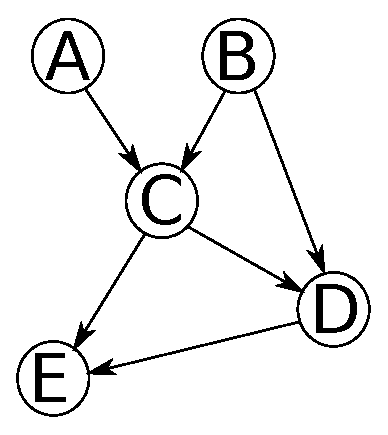
\includegraphics[width=.6\textwidth]{bn1}
    \end{center}
    \column[c]{9cm}
	$p(A,B,C,D,E) = p(A)p(B)p(C|A,B)p(D|B,C)p(E|C,D)$
    \end{columns}
    \textbf{Inference}: Evaluate the probability distribution over some set of variables, given values of another set of variables
    Ex: $p(A|C=c)$?  (binary variables)
    
    \only<2>{
    \textbf{Naive}:
    \begin{align*}
    p(A,C=c) & =  \sum_{B,D,E}p(A,B,C=c,D,E)\qquad{\text{[16 terms]}} \\
    p(C=c) & =  \sum_{A}p(A,C=c)\qquad{\text{[2 terms]}} \\    
    p(A|C=c) &= \frac{p(A,C=c)}{p(C=c)} \qquad{\text{[2 terms]}}\qquad\rightarrow \text{total terms: $20$}
    \end{align*}
    }
    \only<3>{
    \textbf{More efficiently}:
    \begin{align*}
    p(A,C=c) & =  \sum_{B,D,E}p(A)p(B)p(C=c|A,B)p(D|B,C=c)p(E|C=c,D)\\
    & = \scriptsize{\sum_B p(A)p(B)p(C=c|A,B)\sum_D p(D|B,C=c) \sum_E p(E|C=c,D)}\\
    & = \sum_B p(A)p(B)p(C=c|A,B) \qquad [4 \text{ terms}]
    \end{align*}
    }    
\end{frame}


\subsection{Markov Random Fields}


\begin{frame}
	\frametitle{Markov Random Fields}
	\framesubtitle{Undirected graphical models}
    \begin{description}
    \item[Factorization]: over maximal cliques (fully connected subgraphs)
    \end{description}
    \begin{align*}
    p(\mathbf{x})&=\frac{1}{Z}\prod_C \psi_C(\mathbf{x}_C)
    &
    Z = \sum_\mathbf{x}\prod_C \psi_C(\mathbf{x}_C)
    \end{align*}
    where $\psi_C(\mathbf{x}_C)$ is the potential over clique $C$ and
    $Z$ is the partition function
     \begin{description}
    \item[Energy models]: $\psi_C(\mathbf{x}_C) = \exp(-E(\mathbf{x}_C))$\\
    Lower energy $E$ $\rightarrow$ Higher probability $p$\\
    Higher energy $E$ $\rightarrow$ Lower probability $p$
  \end{description}
  
\end{frame} 


\begin{frame}
	\frametitle{Markov Random Fields}
	\framesubtitle{Undirected graphical models}
    \begin{description}
    \item[Conditional Independences] Easier! If $A$ and $B$ become disconnected after removing $C$
    $$A\indep B | C$$
    \vspace{-.5cm}
      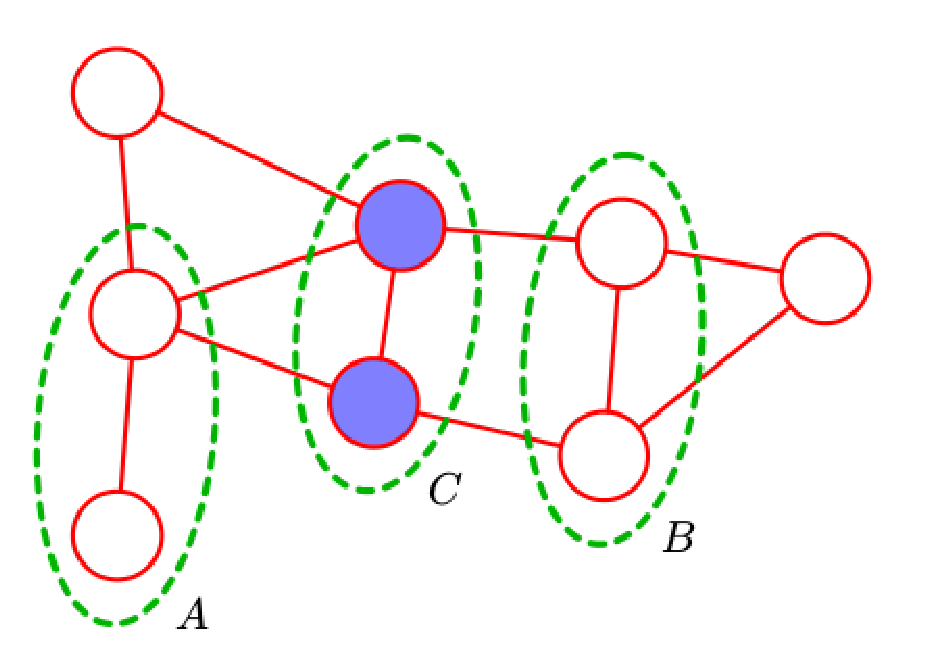
\includegraphics[width=.5\textwidth]{indepmrf}
  \end{description}
  
\end{frame} 


 \begin{frame}
 	\frametitle{Markov Random Fields}
 	\framesubtitle{Undirected graphical models}
     Example: image denoising as an inference task ($x_i\in\{\pm 1\}, y_i\in\{\pm 1\}$)
      \begin{center}
     %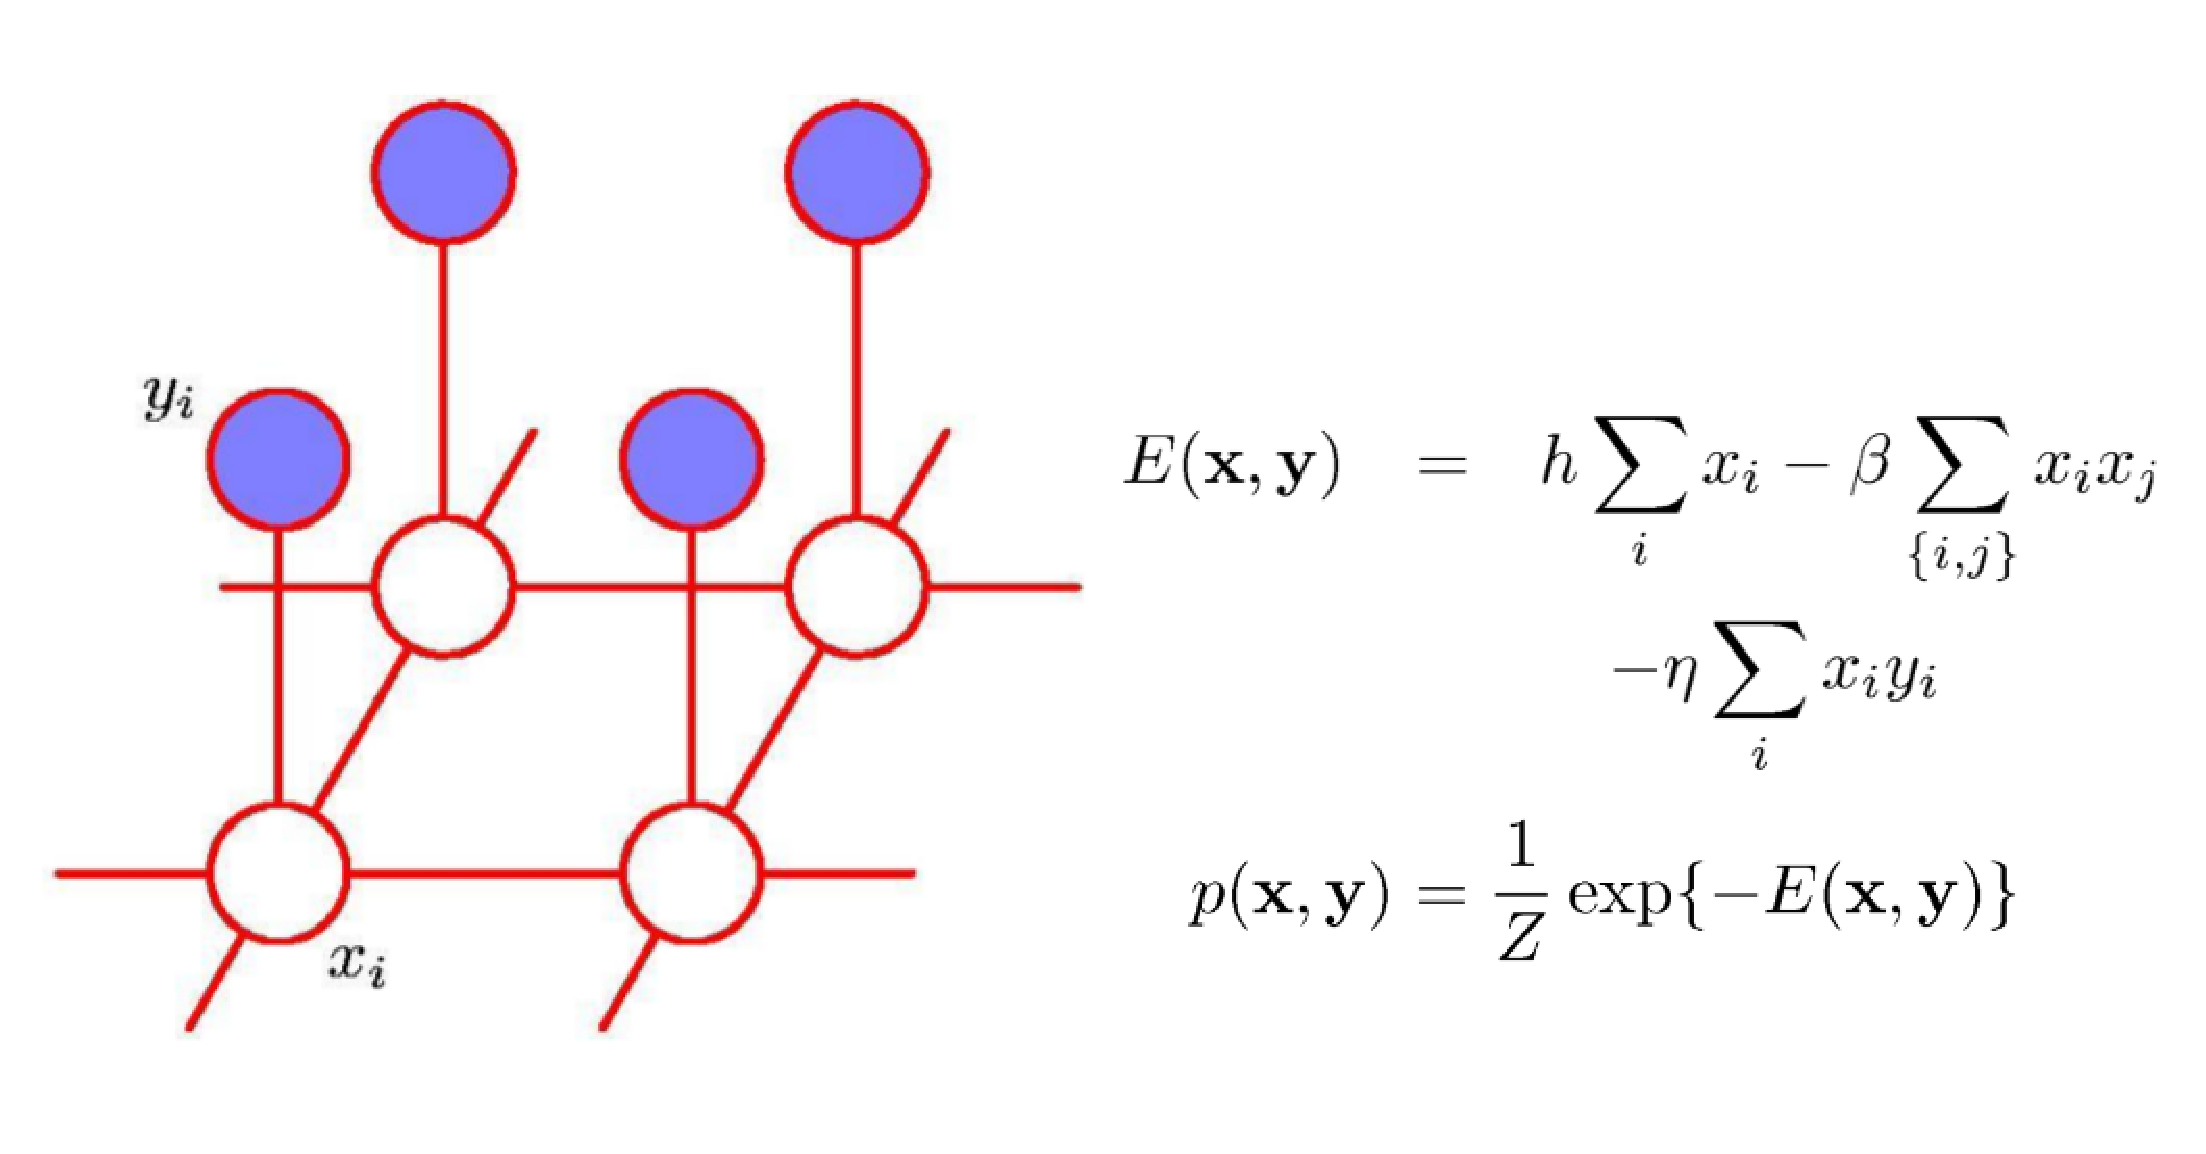
\includegraphics[width=\textwidth]{MRF2}
     \includegraphics[width=.4\textwidth]{MRFWEB}
     \end{center}
     $$E(\mathbf{x},\mathbf{y}) = h\sum_i x_i - \beta\sum_{i,j}x_ix_j - \eta\sum_i x_iy_i$$
     $$p(\mathbf{x},\mathbf{y}) = \frac{1}{Z}\exp\{-E(\mathbf{x},\mathbf{y})\}$$
 \end{frame} 
 
 
 \begin{frame}
 	\frametitle{Markov Random Fields}
 	\framesubtitle{Undirected graphical models}
     Example: image denoising as an inference task
      \begin{center}
    % 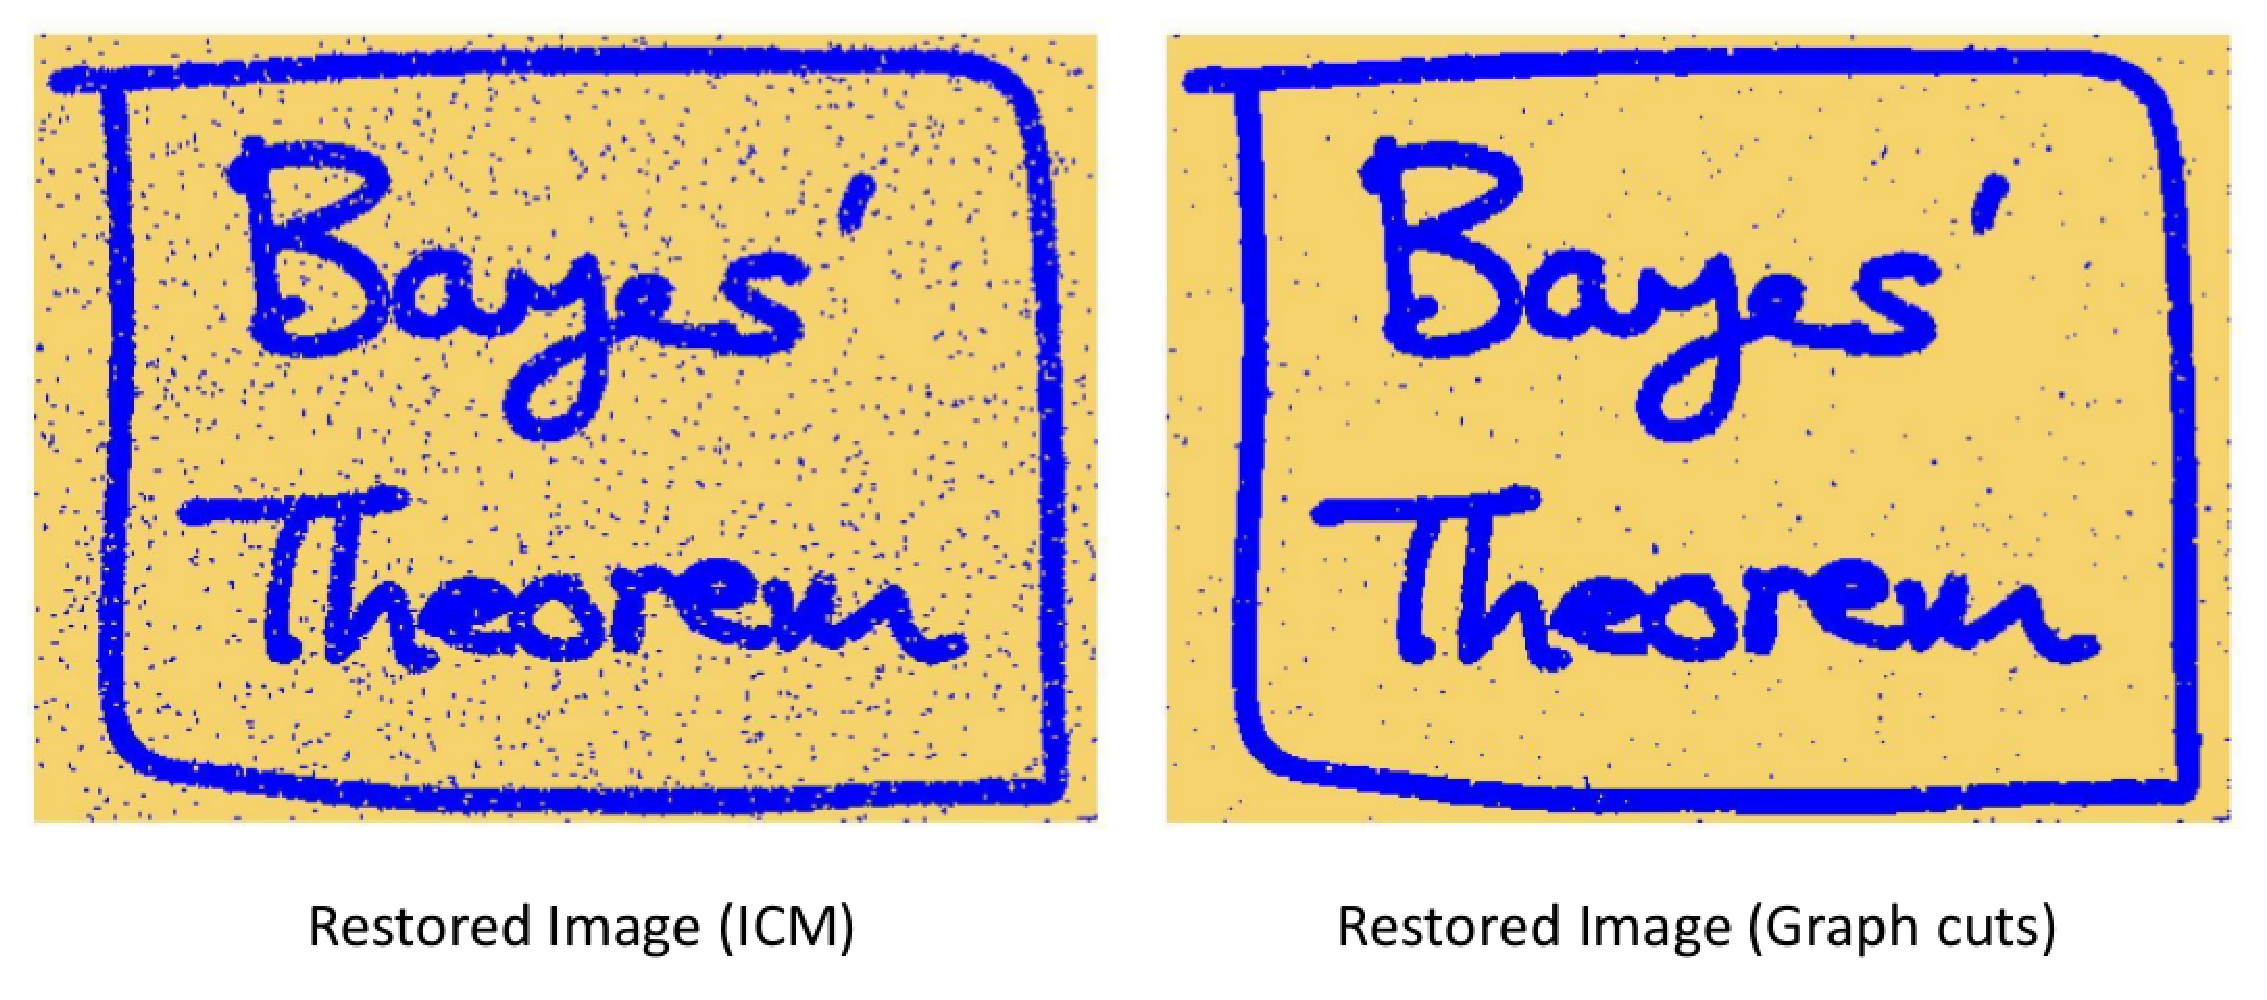
\includegraphics[width=\textwidth]{MRF3}
     \includegraphics[width=\textwidth]{img49.jpg}
        \begin{description}
    \item[Left]: original image
    \item[Middle]: corrupted image (with $p=0.1$ changes pixel)
    \item[Right]: one local minima found over the energy landscape
    \end{description}

     \end{center}
 \end{frame} 

\begin{frame}
	\frametitle{Markov Random Fields}
	\framesubtitle{Inference on a chain}
	A chain of $T$ variables, each having $K$ possible values
    \begin{center}
    \includegraphics[width=.6\textwidth]{chain0}
    \end{center}
    \begin{description}
    \item[Joint probability distribution]:
    \begin{align*}
    p(\mathbf{x})&=\frac{1}{Z}\psi_{1,2}(x_1,x_2)\psi_{2,3}(x_2,x_3) \hdots
       \psi_{T-1,T}(x_{T-1},x_T)
           \end{align*}
    \item[Estimate single-node marginal] $p(x_t)$:
    \begin{align*}
        p(x_t) & = \sum_{x_1}\hdots\sum_{x_{t-1}}\sum_{x_{t+1}}\hdots\sum_{x_T}p(\mathbf{x})
    \end{align*}
	Naive summation has complexity $\mathcal{O}(K^T)$
    \end{description}
  \end{frame} 

\begin{frame}
	\frametitle{Markov Random Fields}
	\framesubtitle{Inference on a chain}
    \begin{center}
    \includegraphics[width=.7\textwidth]{chain1}
    \end{center}
    \begin{align*}
    p(x_t) & = \frac{1}{Z}\underbrace{\left[ \sum_{x_{t-1}}\psi_{t-1,t}(x_{t-1},x_t)\hdots
        \left[ \sum_{x_1}\psi_{1,2}(x_1,x_2)\right] \hdots \right]}_{\mu_\alpha(x_t)}\cdot\\
    &\underbrace{\left[\sum_{x_{t+1}}\psi_{t,t+1}(x_t,x_{t+1})\hdots\left[
    \sum_{x_T}\psi_{T-1,T}(x_{T-1},x_T)
    \right]\hdots\right]}_{\mu_\beta(x_t)}
    \end{align*}
  \end{frame} 

\begin{frame}
	\frametitle{Markov Random Fields}
	\framesubtitle{Inference on a chain}
    \begin{center}
    \includegraphics[width=.6\textwidth]{chain2}
    \end{center}
    \begin{align*}
    \mu_\alpha(x_t) & = 
    \sum_{x_{t-1}}\psi_{t-1,t}(x_{t-1},x_t)\left[\sum_{x_{t-2}}\hdots\right]\\
        & = 
    \sum_{x_{t-1}}\psi_{t-1,t}(x_{t-1},x_t)\mu_\alpha(x_{t-1})
    \end{align*}
    \begin{align*}
    \mu_\beta(x_t) & = 
    \sum_{x_{t+1}}\psi_{t,t+1}(x_{t},x_{t+1})\left[\sum_{x_{t+2}}\hdots\right]\\
        & = 
    \sum_{x_{t+1}}\psi_{t,t+1}(x_{t},x_{t+1})\mu_\beta(x_{t+1})
    \end{align*}
  \end{frame} 

\begin{frame}
	\frametitle{Markov Random Fields}
	\framesubtitle{Inference on a chain}
    \begin{center}
    \includegraphics[width=.6\textwidth]{chain2}
    \end{center}
    \begin{align*}
    \mu_\alpha(x_2) & = \sum_{x_1}\psi_{1,2}(x_1,x_2) &
    \mu_\alpha(x_{T-1}) & = \sum_{x_T}\psi_{T-1,T}(x_{T-1},x_T)\\
    Z_{x_t} & =\sum_{x_t}\mu_\alpha(x_t)\mu_\beta(x_t)
    \end{align*}
\vspace{-.5cm}
    \begin{block}{Computing local marginals in a chain}
     \begin{enumerate}
     \item Compute forward messages $\mu_\alpha(x_t)$
	\item Compute backward messages $\mu_\beta(x_t)$
      \item Compute $p(x_t)=\frac{1}{Z_{x_t}}\mu_{\alpha}(x_t)\mu_\beta(x_t)$, $Z_{x_t}$ sum over all $x_t$ values
\item Complexity $\mathcal{O}(K^T) \rightarrow \mathcal{O}(TK^2)$
     \end{enumerate}
    \end{block}
  \end{frame} 

\subsection{Factor graphs}
\begin{frame}
	\frametitle{Bipartite Factor Graphs}
	\framesubtitle{General class of graphical models}
    \begin{description}
    \item[Factor graphs] subsume both Bayesian networks and MRFs
    \end{description}
    \begin{center}
    \includegraphics[width=.3\textwidth]{factorgraph}
    \end{center}
    Factorization: $
    p(\mathbf{x}) = \frac{1}{Z}f_a(x_1,x_2)f_b(x_1,x_2)f_c(x_2,x_3)f_d(x_3)$
    \bi
    \item MRF: factors correspond to maximal cliques potentials $\mathbf{x}_s$
    \begin{center}
    \includegraphics[width=.6\textwidth]{MRFtoFG}
    \end{center}
    \ei
\end{frame}

\begin{frame}
	\frametitle{Bipartite Factor Graphs}
	\framesubtitle{General class of graphical models}
    \begin{description}
    \item[Factor graphs] subsume both Bayesian networks and MRFs
    \end{description}
    \begin{center}
    \includegraphics[width=.3\textwidth]{factorgraph}
    \end{center}
    Factorization: $
    p(\mathbf{x}) = \frac{1}{Z}f_a(x_1,x_2)f_b(x_1,x_2)f_c(x_2,x_3)f_d(x_3)$
    \bi
    \item BN: factors correspond to conditional probability tables
    \begin{center}
    \includegraphics[width=.55\textwidth]{BNtoFG}
    \end{center}
    \ei
\end{frame}

\subsection{Inference and message passing algorithms}

\begin{frame}
	\frametitle{Bipartite factor graphs}
    \framesubtitle{Inference}
    \begin{block}{Sum-Product (belief propagation) algorithm}
    \bi
    \item Generic algorithm to compute local marginals in a factor graph
    \item Rediscovered several times: Gallager, J. Pearl, Kalman, ...
    \ei
    \end{block}
    Iterates the following messages:
    \begin{description}
    \item [variable to factor]:
    \begin{align*}
    \mu_{i\rightarrow a}(x_i) = \prod_{b\in\mathcal{N}(i)\backslash a}\mu_{b\rightarrow i}(x_i)
    \end{align*}
    \end{description}
    \begin{center}
    \includegraphics[width=.2\textwidth]{bp}
    \end{center}
\end{frame}


\begin{frame}
	\frametitle{Bipartite factor graphs}
    \framesubtitle{Inference}
    \begin{block}{Sum-Product (belief propagation) algorithm}
    \bi
    \item Generic algorithm to compute local marginals in a factor graph
    \item Rediscovered several times: Gallager, J. Pearl, Kalman, ...
    \ei
    \end{block}
    Iterates the following messages:
    \begin{description}
    \item [factor to variable]
    \begin{align*}
    \mu_{a\rightarrow i}(x_i) = \sum_{\mathbf{x}_a\backslash \{i\}}f_a(\mathbf{x}_a)\prod_{j\in\mathcal{N}(a)\backslash i}\mu_{j\rightarrow a}(x_j)
    \end{align*}
    \end{description}
    \begin{center}
    \includegraphics[width=.2\textwidth]{bp2}
    \end{center}
\end{frame}

\begin{frame}
	\frametitle{Bipartite factor graphs}
    \framesubtitle{Inference}
    \begin{description}
    \item[Example of inference using Belief Propagation (root node is $x_3$)]
        \end{description}
 %    \begin{columns}
 %   \column[c]{6cm}
\begin{center}
\includegraphics[width=.4\textwidth]{bpex1}
\end{center}
 %   \column[c]{5cm}
    \begin{align*}
    p(\mathbf{x})& \propto f_a(x_1,x_2)f_b(x_2,x_3)f_c(x_2,x_4)
    \end{align*}
 %\end{columns}
\end{frame}

 \begin{frame}
	\frametitle{Bipartite factor graphs}
    \framesubtitle{Example of inference using Belief Propagation (from leaves to root)}
%     \begin{columns}
%    \column[c]{6cm}
\begin{center}
	\only<1>{\includegraphics[width=.3\textwidth]{bpex_1}}
	\only<2>{\includegraphics[width=.3\textwidth]{bpex_2}}
	\only<3>{\includegraphics[width=.3\textwidth]{bpex_3}}
	\only<4>{\includegraphics[width=.3\textwidth]{bpex_4}}
	\only<5>{\includegraphics[width=.3\textwidth]{bpex_5}}
	\only<6>{\includegraphics[width=.3\textwidth]{bpex_6}}
\end{center}
%    \column[c]{5cm}
    \begin{align*}
    \only<1->{\mu_{x_1\rightarrow f_a}(x_1) & = \texttt{ones}}\\
    \only<2->{\mu_{f_a\rightarrow x_2}(x_2) & = \sum_{x_1}f_a(x_1,x_2)\mu_{x_1\rightarrow f_a}(x_1)}\\
    \only<3->{\mu_{x_4\rightarrow f_c}(x_4) & = \texttt{ones}}\\
    \only<4->{\mu_{f_c\rightarrow x_2}(x_2) & = \sum_{x_4}f_c(x_2,x_4)}\\
    \only<5->{\mu_{x_2\rightarrow f_b}(x_2) & = \mu_{f_a\rightarrow x_2}(x_2)\mu_{f_c\rightarrow x_2}(x_2)} \\
    \only<6->{\mu_{f_b\rightarrow x_3}(x_3) & = \sum_{x_2}f_b(x_2,x_3)\mu_{x_2\rightarrow f_b}(x_2) }
    \end{align*}
% \end{columns}
\end{frame}

  \begin{frame}
	\frametitle{Bipartite factor graphs}
    \framesubtitle{Example of inference using Belief Propagation (from root to leaves)}
%     \begin{columns}
%    \column[c]{6cm}
\begin{center}
	\only<1>{\includegraphics[width=.3\textwidth]{bpex_21}}
	\only<2>{\includegraphics[width=.3\textwidth]{bpex_22}}
	\only<3>{\includegraphics[width=.3\textwidth]{bpex_23}}
	\only<4>{\includegraphics[width=.3\textwidth]{bpex_24}}
	\only<5>{\includegraphics[width=.3\textwidth]{bpex_25}}
	\only<6>{\includegraphics[width=.3\textwidth]{bpex_26}}
\end{center}
%    \column[c]{5cm}
    \begin{align*}
    \only<1->{\mu_{x_3\rightarrow f_b}(x_3) & =  \texttt{ones}}\\
    \only<2->{\mu_{f_b\rightarrow x_2}(x_2) & = \sum_{x_3}f_b(x_2,x_3)}\\
    \only<3->{\mu_{x_2\rightarrow f_a}(x_2) & = \mu_{f_b\rightarrow x_2}(x_2)\mu_{f_c\rightarrow x_2}(x_2)} \\
    \only<4->{\mu_{f_a\rightarrow x_1}(x_1) & = \sum_{x_2}f_a(x_1,x_2)\mu_{x_2\rightarrow f_a}(x_2) }\\
    \only<5->{\mu_{x_2\rightarrow f_c}(x_2) & = \mu_{f_a\rightarrow x_2}(x_2)\mu_{f_b\rightarrow x_2}(x_2)} \\
    \only<6->{\mu_{f_c\rightarrow x_4}(x_4) & = \sum_{x_2}f_c(x_2,x_4)\mu_{x_2\rightarrow f_c}(x_2) }
    \end{align*}
% \end{columns}
\end{frame}



  \begin{frame}
	\frametitle{Bipartite factor graphs}
    \framesubtitle{Example of inference using Belief Propagation (from root to leaves)}
%     \begin{columns}
%    \column[c]{6cm}
\begin{center}
	\only<1>{\includegraphics[width=.3\textwidth]{bpex_21}}
	\only<2>{\includegraphics[width=.3\textwidth]{bpex_22}}
	\only<3>{\includegraphics[width=.3\textwidth]{bpex_23}}
	\only<4>{\includegraphics[width=.3\textwidth]{bpex_24}}
	\only<5>{\includegraphics[width=.3\textwidth]{bpex_25}}
	\only<6>{\includegraphics[width=.3\textwidth]{bpex_26}}
\end{center}
%    \column[c]{5cm}
After the two passes, any single variable marginal can be computed taking the product of incoming messages and normalizing
    \begin{align*}
	Z_{x_2} & = \sum_{x_2} \mu_{f_a\rightarrow x_2}(x_2)\mu_{f_b\rightarrow x_2}(x_2)\mu_{f_c\rightarrow x_2}(x_2) \\
	p(x_2) & = \frac{1}{Z_{x_2}}\mu_{f_a\rightarrow x_2}(x_2)\mu_{f_b\rightarrow x_2}(x_2)\mu_{f_c\rightarrow x_2}(x_2)
    \end{align*}
% \end{columns}
\end{frame}


  \begin{frame}
	\frametitle{Probabilistic Inference}
    \framesubtitle{Hidden Markov models and Linear Gaussian state-space models}
%     \begin{columns}
%    \column[c]{6cm}
\begin{center}
\includegraphics[width=.6\textwidth]{hmm}
\end{center}
$$p(X_{1,\hdots,T},Y_{1,\hdots,T}) = p(X_1)p(Y_1|X_1)\prod_{t=2}^T p(X_t|X_{t-1})p(Y_t|X_t)$$
\begin{itemize}
\item In HMMs, the states $X_t$ are discrete
\item In linear Gaussian SSMs, the states are real Gaussian vectors
\item Both HMMs and SSMs can be represented as singly connected DAGs
\item The \textbf{forward-backward algorithm} in HMMs and the \textbf{Kalman smoothing algorithm} in SSMs are both 
	instances of belief propagation / factor graph representation
\end{itemize}

\end{frame}

 
\begin{frame}
	\frametitle{Bipartite factor graphs}
    \framesubtitle{Belief Propagation algorithm}
    \begin{block}{Sum-Product algorithm}
    \bi
    \item Generic algorithm to compute local marginals in a factor graph
    \item Sum-Product is exact on tree graphs
    \item Can be an approximate algorithm on loopy graphs (LBP)
    \item Convergence is not guaranteed
    \item Variational interpretation:
    fixed points of LBP are stationary points of a free energy function
    \item Exact inference in loopy graphs
    \bi
    \item Compile the graph into a tree (cluster graph)
    \item Run message passing on it
    \item Complexity exponential in maximum clique size
    \ei
    \ei
    \end{block}
    
\end{frame}

\subsection{Learning Graphical Models}

\begin{frame}
	\frametitle{Learning graphical Models}
    \framesubtitle{Given the graph, learn the parameters}
	\vspace{-.3cm}
	\begin{columns}[T]
	 \column{0.15\textwidth}
	 \includegraphics[width=\textwidth]{g2}
	 \column{0.3\textwidth}
	 $p(X_1)p(X_2|X_1)p(X_3|X_1)p(X_4|X_3)$
	 \column{0.3\textwidth}
	 \begin{table}[!h]
	\begin{tabular}{|l|l|l|l|}
	\hline
	$\theta_2$ & \multicolumn{3}{l|}{$X_2$} \\ \hline
	$X_1$      & 0.2     & 0.3     & 0.5    \\ \hline
	           & 0.1     & 0.6     & 0.3    \\ \hline
	\end{tabular}
	\end{table}
	\par
	\end{columns}
	\small
	\begin{itemize}[<+->]
	\item Assume each variable $X_i$ is discrete and can take on $K_i$ values
	\item The parameters can be represented as 4 tables: $\theta_1$ has $K_1$, $\theta_2$ has entries $K_1\times K_2$, etc...
	\item \textbf{Conditional Probability Tables} (CPTs) with the following semantics:
	$$p(x_1 = k) = \theta_{1,k}, \qquad p(x_2=k'| x_1 = k)	 = \theta_{2,k,k'}$$
	\item
	If node $i$ has $M$ parents, $\theta_i$:
	$M+1$ dimensional table
	
	or $2$-dimensional table with ($\prod_{j\in\text{pa}(i)}K_j\times K_i$) entries by collapsing
 all the states of the parents of node $i$. Note that $\sum_{k'}\theta_{i,k,k'} = 1$
		
	\item Assume a data set $\mathcal{D} = \{ \mathbf{x}^n \}_{n=1}^{N}\qquad$
\only<2->{\color{red} How do we learn $\theta$ from $\mathcal{D}$?}
    	
	\end{itemize}
	
\end{frame}


\begin{frame}
	\frametitle{Learning graphical Models}
    \framesubtitle{Given the graph, learn the parameters}
	\vspace{-.3cm}
	\begin{columns}[T]
	 \column{0.75\textwidth}
	 Assume a data set $\mathcal{D} = \{ \boldsymbol{x}^n \}_{n=1}^{N}\qquad$ \\
	 \vspace{.1cm}
	 How do we learn $\theta$ from $\mathcal{D}$?
	 \column{0.15\textwidth}
	 \includegraphics[width=\textwidth]{g2}
	\end{columns}
	$$p(\boldsymbol{x}|\boldsymbol{\theta})=p(x_1|\theta_1)p(x_2|x_1,\theta_2)p(x_3|x_1,\theta_3)p(x_4|x_3,\theta_4)$$
\vspace{-.35cm}
\begin{itemize}[<+->]
\item Likelihood: $\quad p(\mathcal{D}|\boldsymbol{\theta}) = \prod_{n=1}^N p(\boldsymbol{x}^{(n)}|\boldsymbol{\theta})$
\item Log-Likelihood: $\quad \log p(\mathcal{D}|\boldsymbol{\theta}) = \sum_{n=1}^N\sum_i\log p(x_i^{(n)}|x_{\text{pa(i)}}^{(n)},\theta_i)$
\item This decomposes into sum of functions of $\theta_i$ (optimized separately)
\end{itemize}
\visible<4->{
\begin{columns}[T]
\column{0.5\textwidth}
$$\theta_{i,k,k'} = \frac{n_{i,k,k'}}{\sum_{k''} n_{i,k,k''}}$$
\column{0.5\textwidth}
$n_{i,k,k''}$ is \# times in $\mathcal{D}$ where $x_i=k'$ and $x_{\text{pa(i)}}=k$ ($k$ joint configuration
of the parents)}
\end{columns}
\only<5->{\color{red} ML solution: Simply calculate frequencies!}
\end{frame}



\begin{frame}
	\frametitle{Learning graphical Models}
    \framesubtitle{Maximum Likelihood Learning with Hidden Variables}
	\begin{columns}[T]
	 \column{0.7\textwidth}
	\begin{description}
	\item[Goal]: Maximize parameter log-likelihood given observables
	$$\mathcal{L}(\theta) = \log p(Y|\theta) = \log \sum_{X} p(Y,X|\theta)$$
	\end{description}
	\column{0.25\textwidth}
	\includegraphics[width=.8\textwidth]{g3}
	\end{columns}
	
	\begin{description}
	\item[The Expectation - Maximization (EM) algorithm (intuition)]
	\end{description}
	Iterate between applying the following two steps:
	\begin{itemize}
	\item \textbf{The E-Step}: fill-in the hidden/missing variables
	\item \textbf{The M-Step}: apply complete data learning to filled-in data.
	
		Previous slide formula 	
	\end{itemize}
\end{frame}

\end{document}
